\sectionframe{The Next Step}

\section{The Next Step}

\begin{frame}{Hypothesis}
    Research question 3 remaining: What else can happen?

    \pause
    \vspace{2em}
    Hypothesis:
    \begin{itemize}
        \item Period Adding
    \end{itemize}
\end{frame}

\begin{frame}{What is Period Adding?}
    \begin{columns}
        \begin{column}{.6 \textwidth}
            Between two parameter regions with cycles $\Cycle{L}$ and $\Cycle{R}$ there are parameter regions with:
            \begin{itemize}
                \item The cycle $\Cycle{LR}$ in the middle
                \item The cycle $\Cycle{L^2R}$ between $\Cycle{L}$ and $\Cycle{LR}$
                \item The cycle $\Cycle{LR^2}$ between $\Cycle{LR}$ and $\Cycle{R}$
                \item etc.
            \end{itemize}

            \vspace{1em}
            \onslide<2->{
                The cycles are glued together \\
                $\implies$ The periods add and so do the rotations \\
            }
            \onslide<3->{
                $\implies$ Their ratio $\left(\dfrac{\text{rotations}}{\text{period}}\right)$ follows Farey-Adding
            }
        \end{column}
        \begin{column}{.4 \textwidth}
            \vspace{-3em}
            \begin{figure}
                \centering
                \subfloat{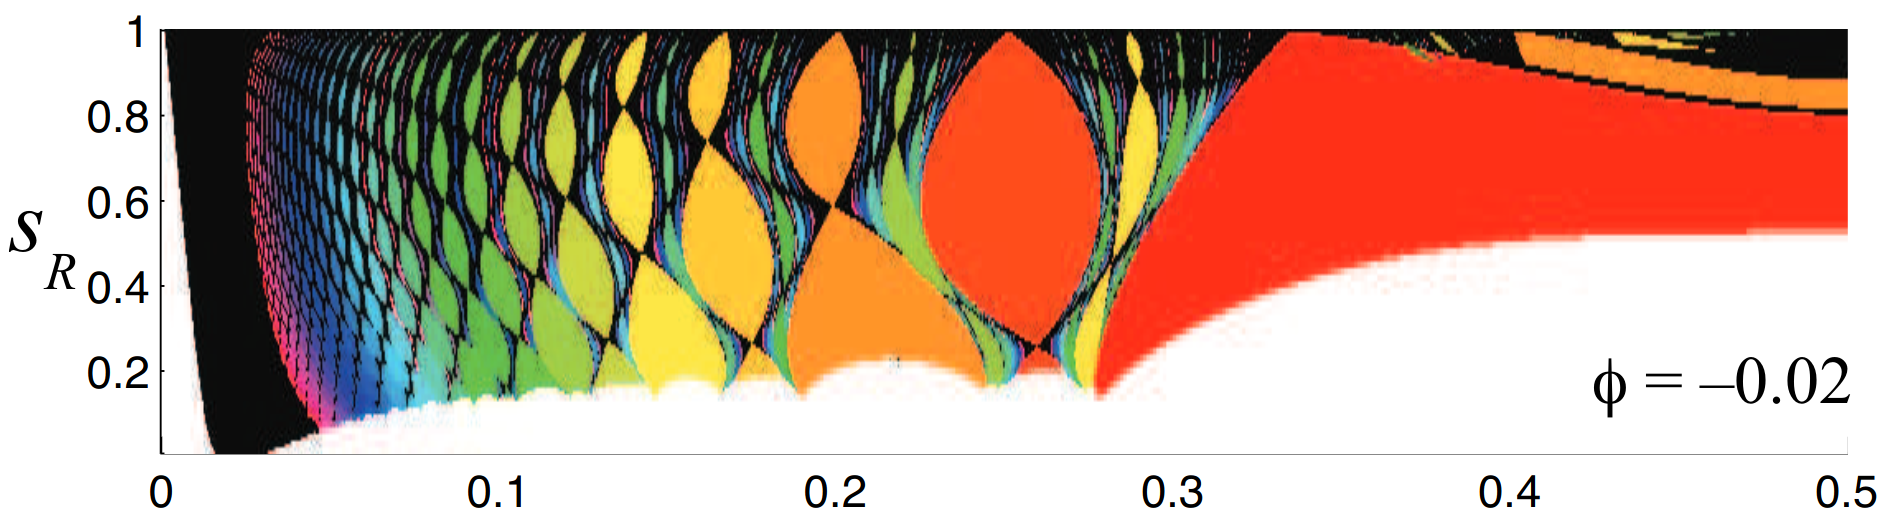
\includegraphics[width=\textwidth]{gfx/tounge_adding.png}}
                \\
                \subfloat{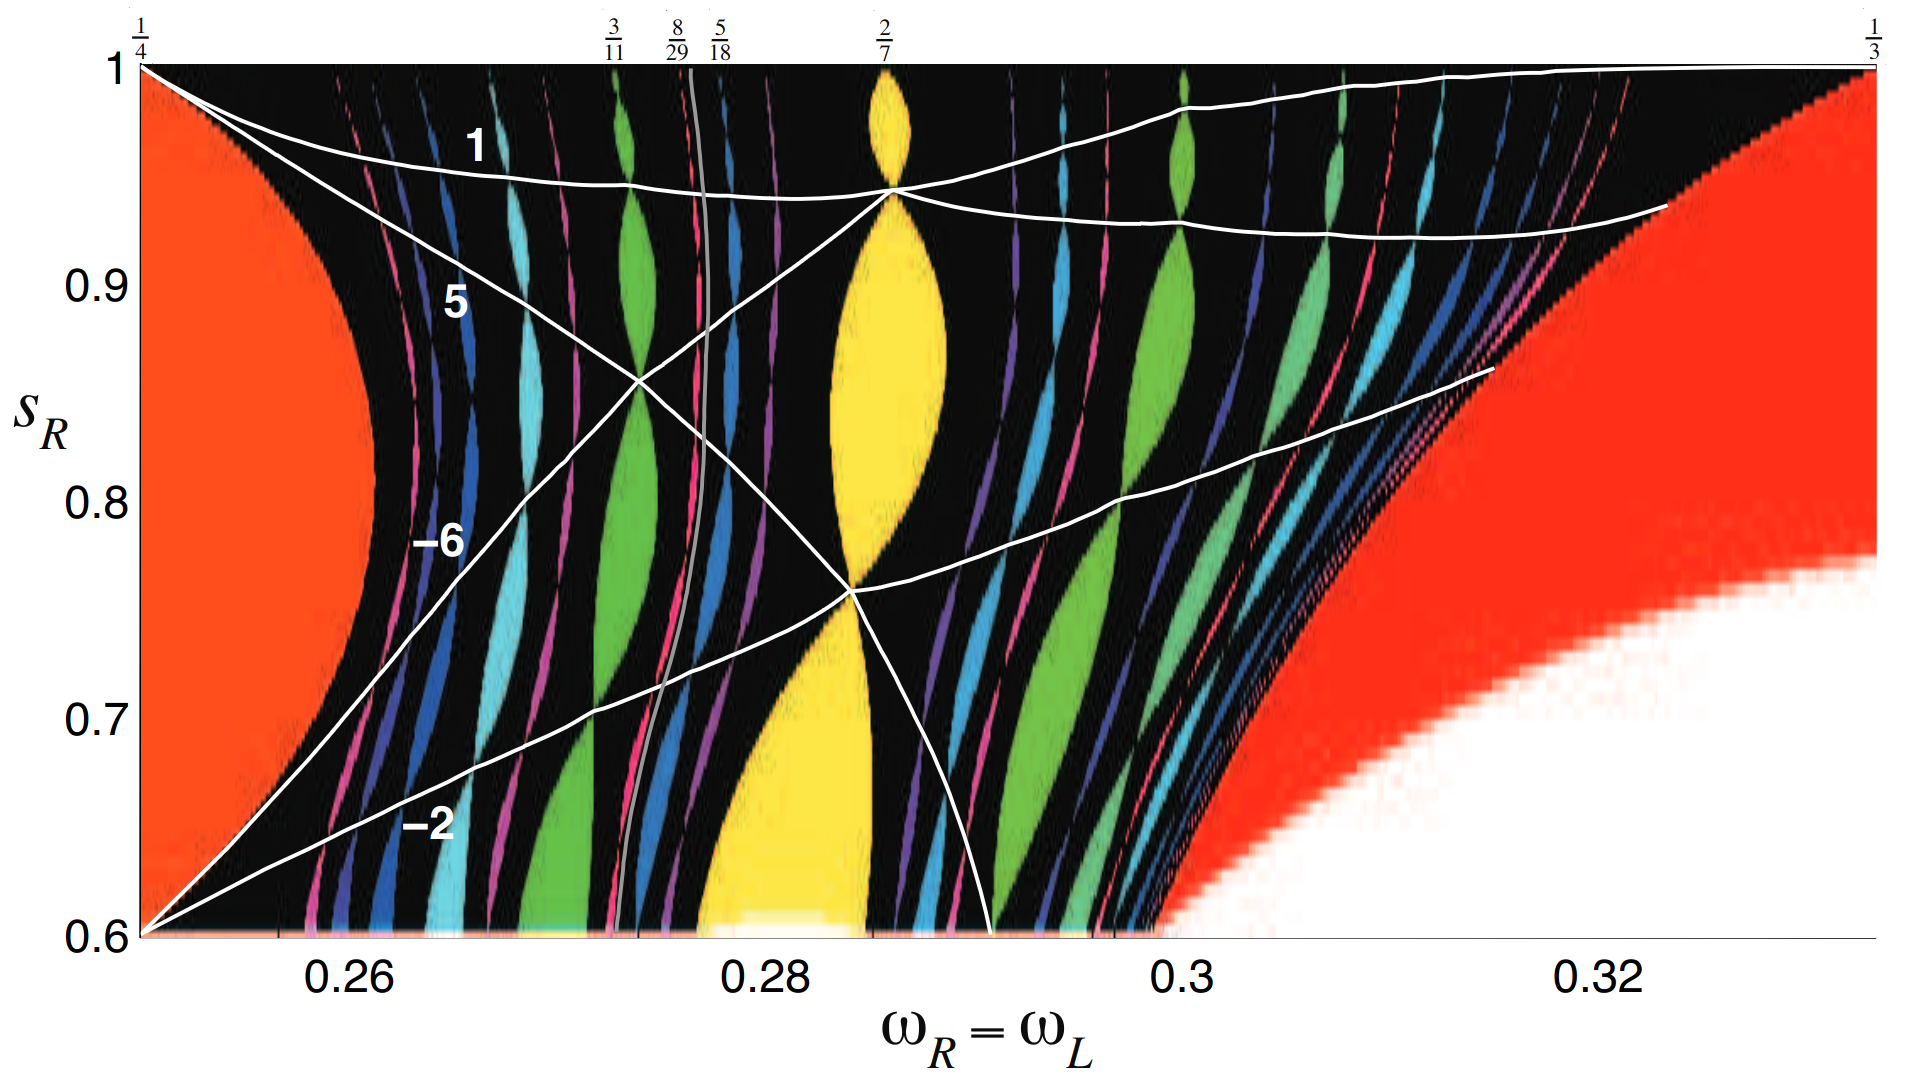
\includegraphics[width=\textwidth]{gfx/tounge_adding_zoomed.png}}
            \end{figure}
            \begin{flushright}
                Pictures from \cite{simpson2010}
            \end{flushright}
        \end{column}
    \end{columns}
\end{frame}

%\begin{frame}{Motivation}
%    \vspace{-2.0em}
%    Full Model:
%    \begin{itemize}
%        \item $\Cycle{\A^x\B^y\C^x\D^y}$
%        \item $\Cycle{\A^x\B^y\C^{x-1}\D^{y+1}}$ and $\Cycle{\A^{x-1}\B^{y+1}\C^x\D^y}$ coexisting
%        \item $\Cycle{\A^{x-1}\B^{y+1}\C^{x-1}\D^{y+1}}$
%    \end{itemize}
%
%    \vspace{1.0em}
%    Halved Model:
%    \begin{itemize}
%        \item $\Cycle{\L^x\R^y}$
%        \item $\Cycle{\L^x\R^y\L^{x-1}\R^{y+1}}$
%        \item $\Cycle{\L^{x-1}\R^{y+1}}$
%    \end{itemize}
%\end{frame}
%
%\begin{frame}{Period-Adding Structures}
%    \vspace{-2.0em}
%    Pattern, period-adding structures follow:
%    \begin{itemize}
%        \item Some cycle $\Cycle{L}$ on the left
%        \item Some cycle $\Cycle{R}$ on the right
%        \item The cycle $\Cycle{LR}$ in the middle
%    \end{itemize}
%
%    \vspace{1.0em}
%    This will hold recursively.
%    \begin{itemize}
%        \item Between $\Cycle{LR}$ and $\Cycle{R}$ there is $\Cycle{LR^2}$
%        \item Between $\Cycle{LR^2}$ and $\Cycle{LR}$ there is $\Cycle{LR^2LR}$
%        \item etc.
%    \end{itemize}
%\end{frame}

\begin{frame}{Searching Period-Adding Structures}
    \begin{itemize}
        \item Investigate the model at different values of the fixed parameters
        \item Look for signs of period adding
        \item Change model if necessary
    \end{itemize}
\end{frame}